\chapter{Dynamic diagrams}
\label{ch:dynamicdiagram}

\section{Core}
\subsection{Initialization of the core from the UI application}
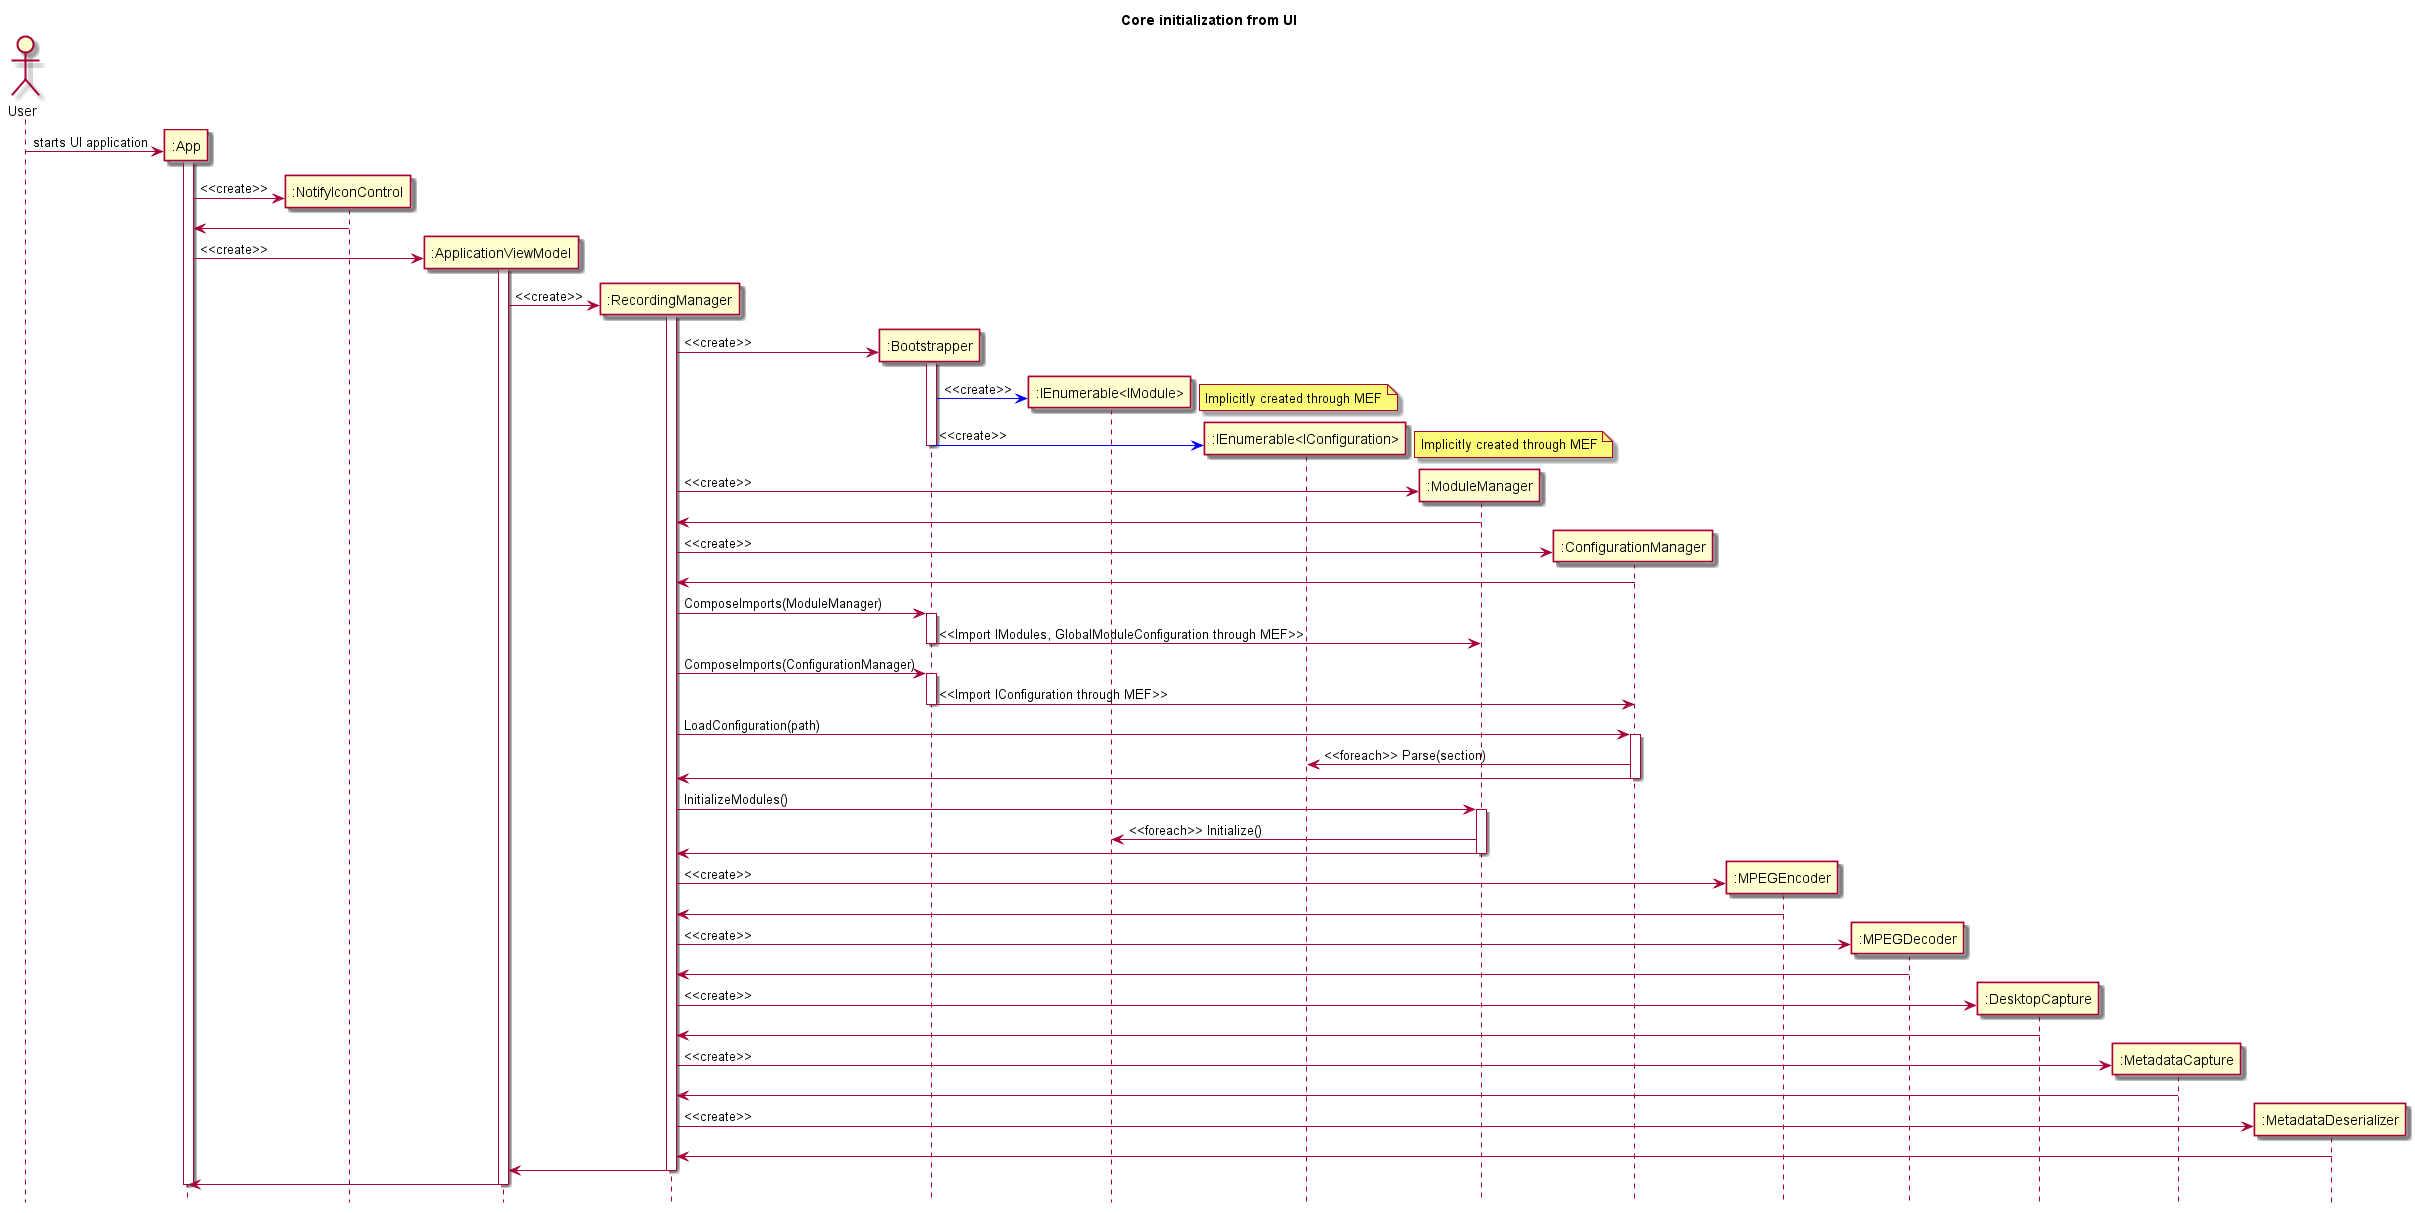
\includegraphics[width=1.1\textwidth]{resources/DynamicDiagrams/InitCore.png}
This diagram depicts the control flow when the user starts the UI application, up to the point where the core is ready for a recording to start.

\subsection{Event flow from keyboard module to the JSON encoder}
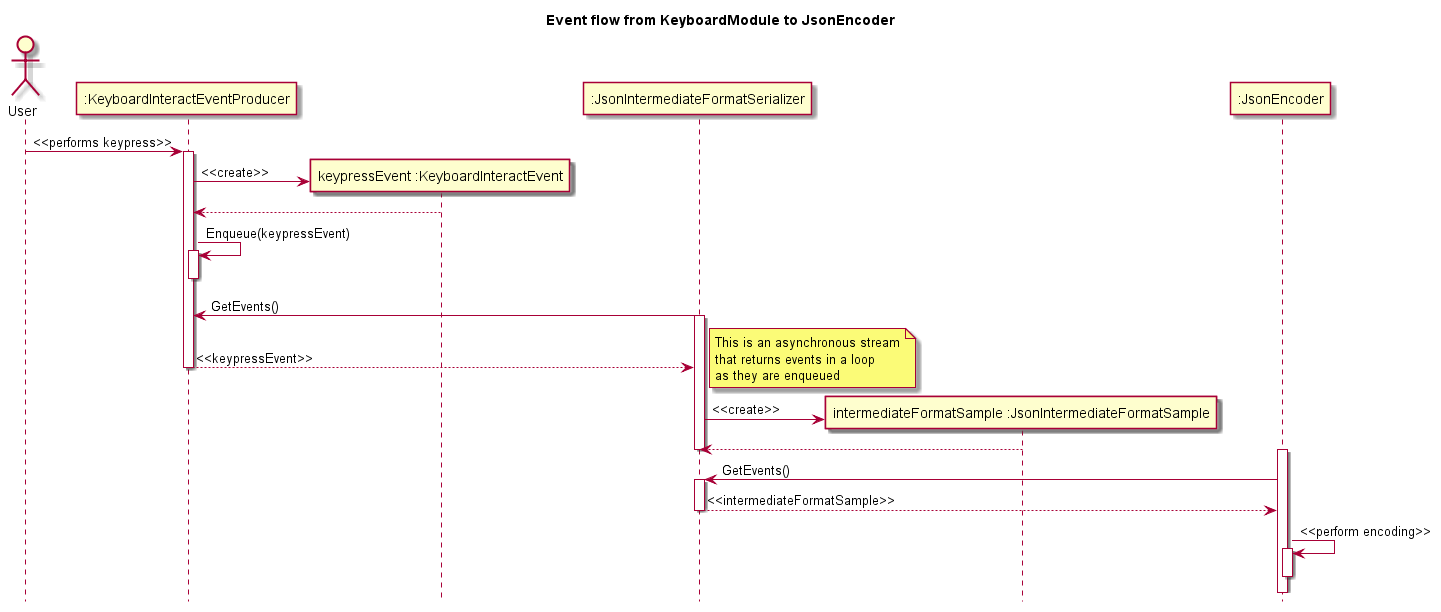
\includegraphics[width=1.1\textwidth]{resources/DynamicDiagrams/EventFlowKeyboardToEncoder.png}
This diagram depicts the control flow when the user presses a keyboard button, up to the point where the event has been encoded into the JSON file during a recording.

\section{Browser Extension}
\subsection{Initialization of the browser extension}
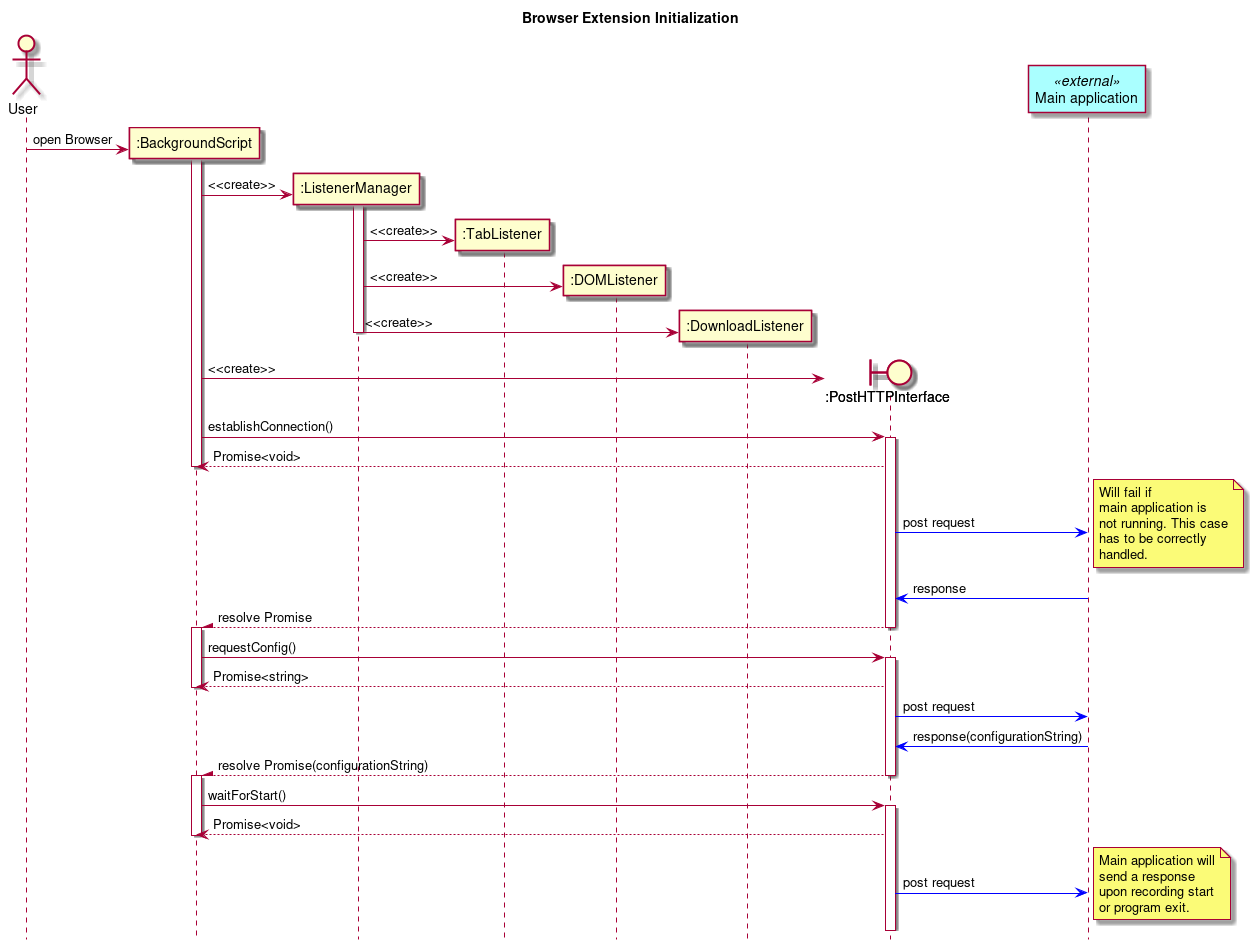
\includegraphics[width=1.0\textwidth]{resources/DynamicDiagrams/InitBrowserEx.png}
This diagram depicts the control flow when the browser is started and the browser extension initialized, up to the point where the browser extension is ready for a recording to start.

\subsection{Capturing a text selection event}
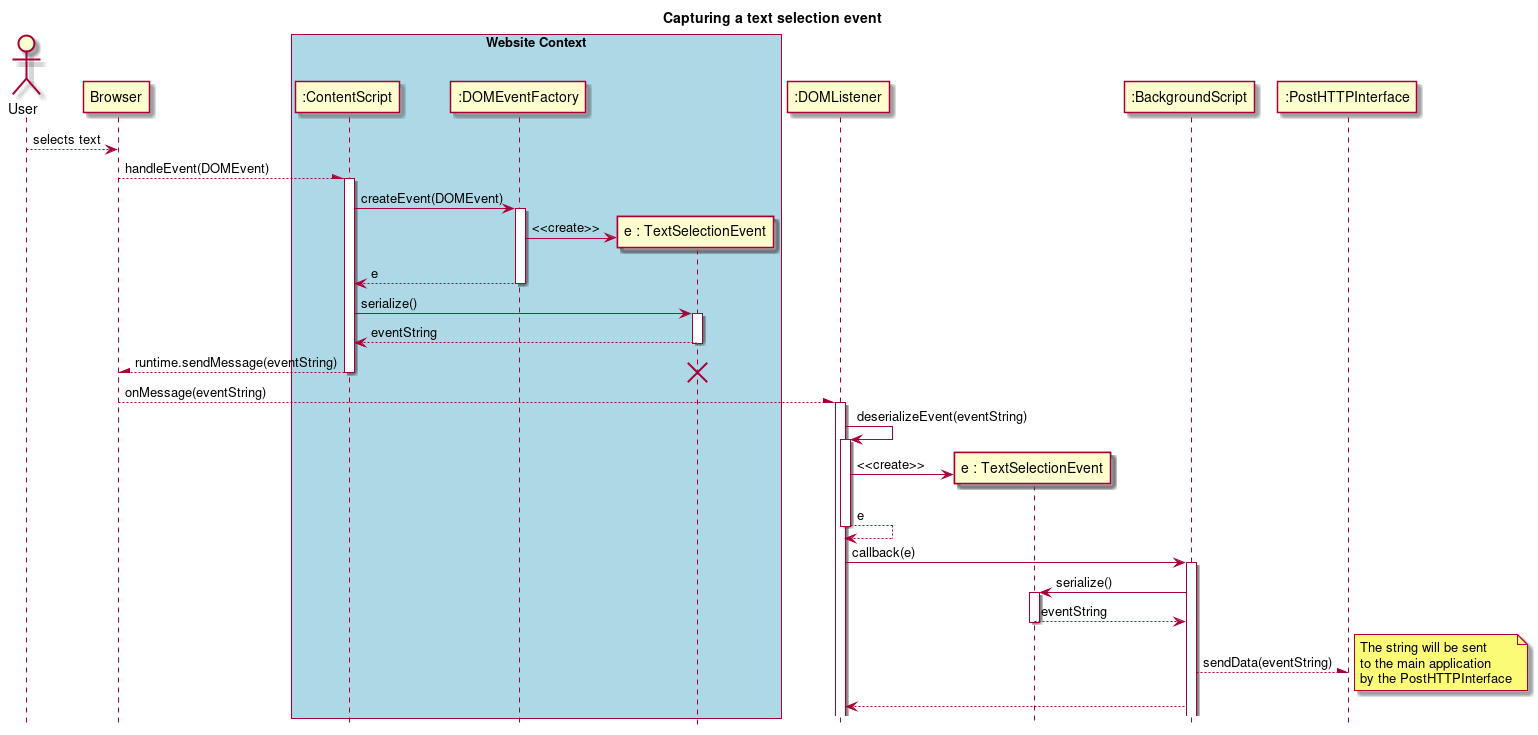
\includegraphics[width=1.0\textwidth]{resources/DynamicDiagrams/CaptureEvent.png}
This diagram depicts the control flow when the browser extension captures a text selection event during a recording. The control flow is described up to the point where the recorded event is handed over to the communication-interface which will attempt to send it to the main application. The control flow for other captured DOM events (meaning events occurring in the website-context) is identical.